\section{Evaluering}

\subsection{Test af sensormodeller}
\begin{frame}
\frametitle{Sammenlignings-skema}
\centering
\begin{columns}
\begin{column}{.49\textwidth}
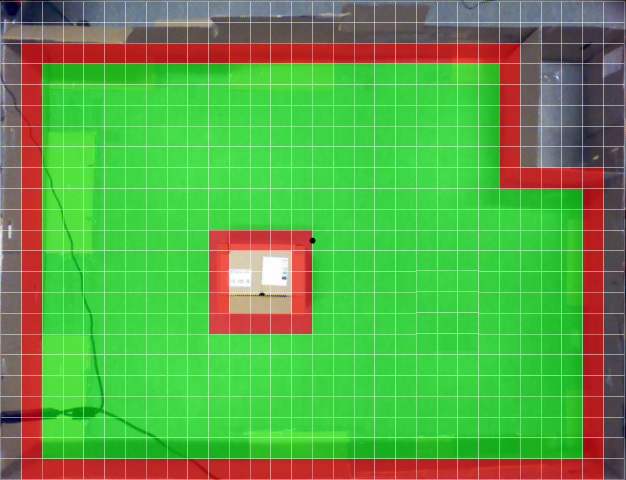
\includegraphics[width=\textwidth]{testresultater/optimalt}
\end{column}
\begin{column}{.49\textwidth}
$P(occupied)$
\begin{itemize}
\item Optaget: $> 0.5$
\item Fri: $< 0.5$
\item Ukendt: $= 0.5$
\end{itemize}
\visible<3->{Maksimal score: 555}
\end{column}
\end{columns}
\pause
\vspace{1em}
\begin{tabular}{ l l | c | c | c |}
\cline{3-5}
&&\multicolumn{3}{| c |}{Optimalt}\\\cline{3-5}
&& Optaget&Fri&Ukendt\\\hline

\multicolumn{1}{| l |}{\multirow{3}{*}{Test}}&
Optaget & $+1$ & {\color{red}$-1$} & {\color{gray}$0$}
\\\cline{2-5}

\multicolumn{1}{|c|}{}&
Fri     & {\color{red}$-1$} & $+1$ & {\color{gray}$0$}
\\\cline{2-5}

\multicolumn{1}{|c|}{}&
Ukendt  & {\color{red}$-1$} & {\color{red}$-1$} & {\color{gray}$0$}
 \\\hline
\end{tabular}
\end{frame}


% SIMPEL SENSOR MODEL
\begin{frame}[fragile]{Simpel sensormodel}
	\begin{columns}
		\begin{column}{0.5\textwidth}
			\begin{itemize}
			\item \textbf{100}/150 opdateringer
			\item \textbf{127}/555 point
			\end{itemize}
			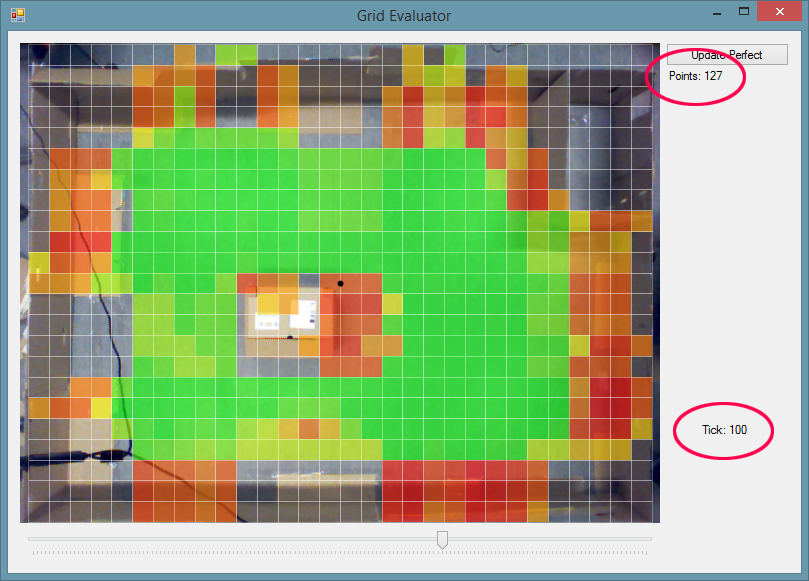
\includegraphics[width=\textwidth]{evaluering/simple3_100.png}
		\end{column}
		\visible<2->
		{\begin{column}{0.5\textwidth}
			\begin{itemize}
			\item \textbf{150}/150 opdateringer
			\item \textbf{193}/555 point
			\end{itemize}
			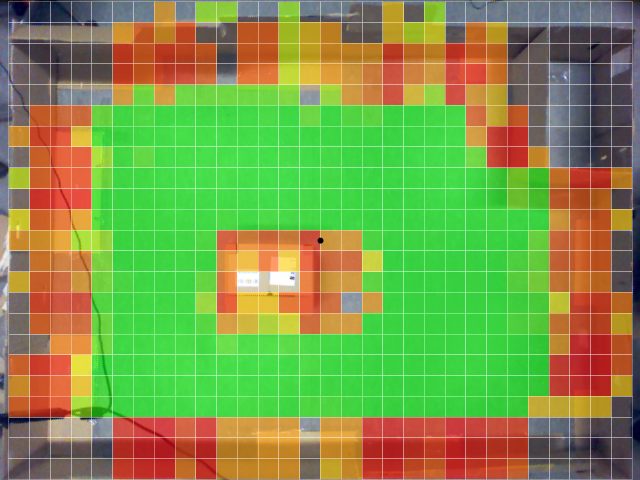
\includegraphics[width=\textwidth]{evaluering/simple3_150.png}
		\end{column}}
\end{columns}
\end{frame}

% GAUSISK SENSOR MODEL
\begin{frame}[fragile]{Gausisk sensormodel}
	\begin{columns}
		\begin{column}{0.5\textwidth}
			\begin{itemize}
			\item \textbf{100}/150 opdateringer
			\item \textbf{295}/555 point
			\end{itemize}
			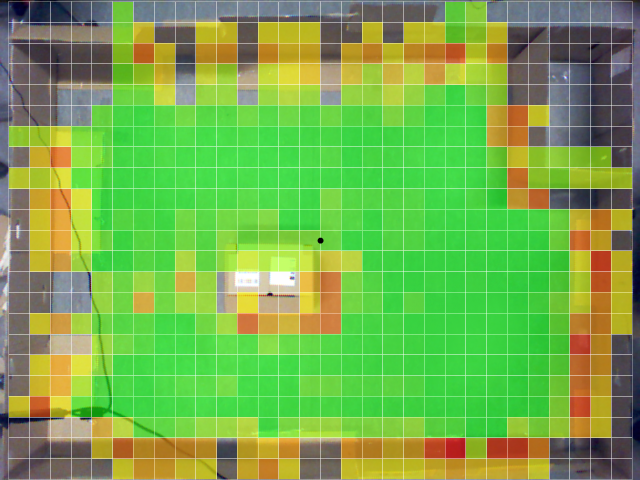
\includegraphics[width=\textwidth]{evaluering/gauss3_100.png}
		\end{column}
		\visible<2->
		{\begin{column}{0.5\textwidth}
			\begin{itemize}
			\item \textbf{150}/150 opdateringer
			\item \textbf{337}/555 point
			\end{itemize}
			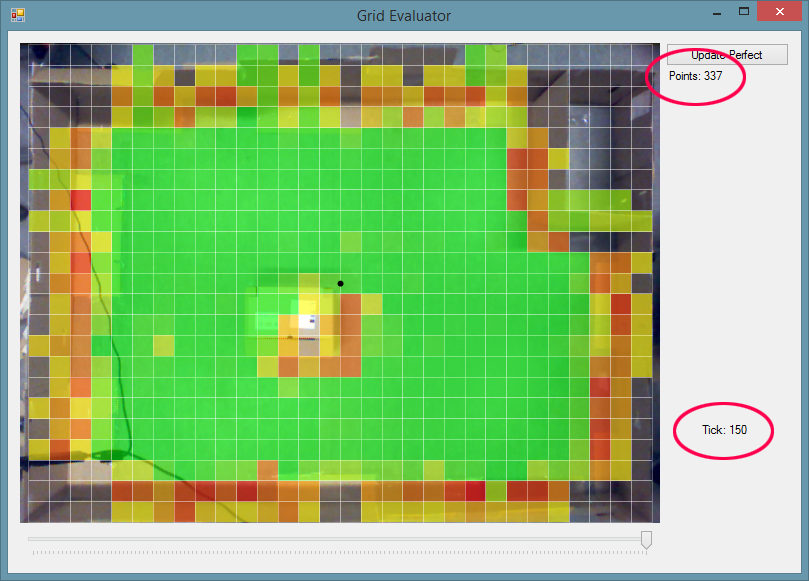
\includegraphics[width=\textwidth]{evaluering/gauss3_150.png}
		\end{column}}
\end{columns}
\end{frame}

% SAMMENLIGNING AF SENSOR MODELLER
\begin{frame}[fragile]{Sammenligning af modeller}
	\begin{columns}
		\begin{column}{0.45\textwidth}
			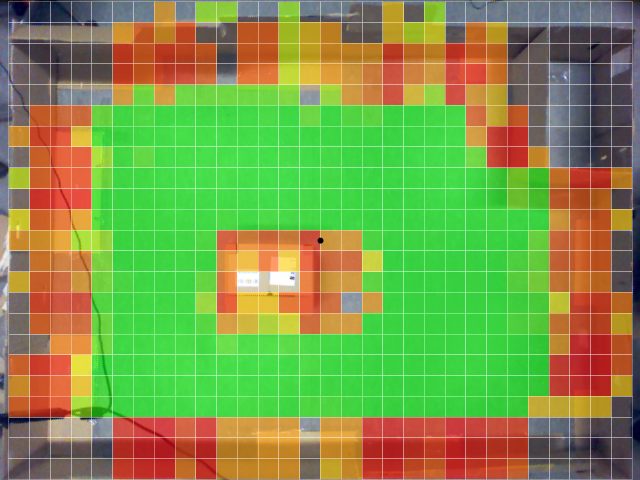
\includegraphics[width=\textwidth]{evaluering/simple3_150.png}
		\end{column}
		\begin{column}{0.45\textwidth}
			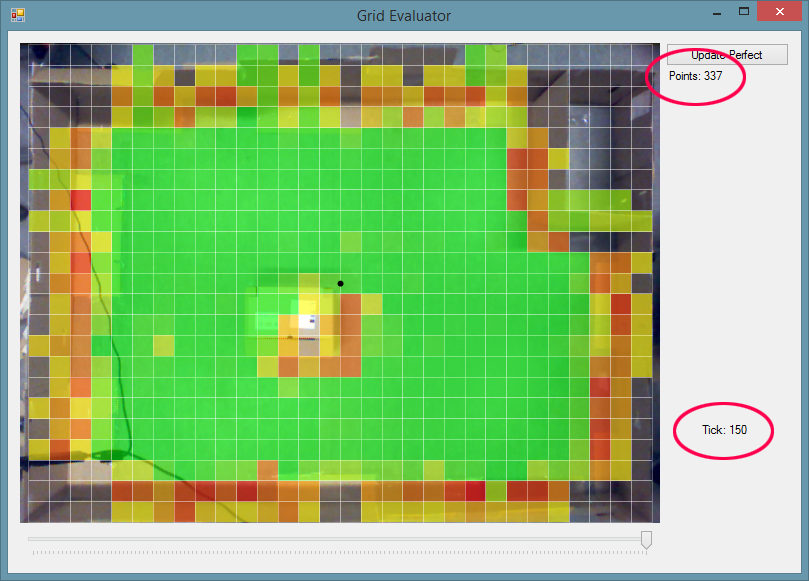
\includegraphics[width=\textwidth]{evaluering/gauss3_150.png}
		\end{column}
	\end{columns}
	\vspace{-0.5em}
	\begin{center}
	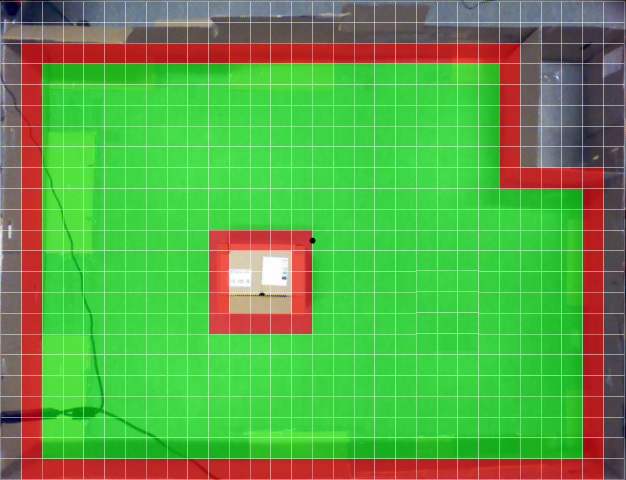
\includegraphics[width=0.45\textwidth]{testresultater/optimalt}
	\end{center}
\end{frame}

\subsection{Problemstillinger \& Forbedringer}

\begin{frame}
\frametitle{Navigation}
Robotten roterer ikke korrekt, hvilket medfører:
\begin{itemize}
\item afvigelse fra den planlagte rute.
\item kollision med kassen i testmiljøet.
\item opdatering af nabocelle istedet for den ønskede celle.
\item robotten er ikke altid orienteret i 90$^\circ$ ved opdatering.
\end{itemize}
\pause
Robotten forespørger kun sin position indtil den er \textit{tilpas} tæt på sin destination.
Den når derfor ikke altid sin destination.
\end{frame}

\begin{frame}
\frametitle{Konstruktion}
\textit{Måletårnet} er placeret forskudt ift. det punkt der spores.\\
Denne konstruktion har medført:
\begin{itemize}
\item øget kompleksitet af kode.
\item en større robot konstruktion.
\item problemer i forhold til robottens bagende.
\end{itemize}
\end{frame}

\begin{frame}
\frametitle{Omgivelser}
\begin{itemize}
\item PC'en der planlægger robottens rute gør udelukkende dette med udgangspunkt i occupancy grid.
\item Robottens sensorer anvendes ikke under navigationen.
\end{itemize}
\centering
\visible<2->{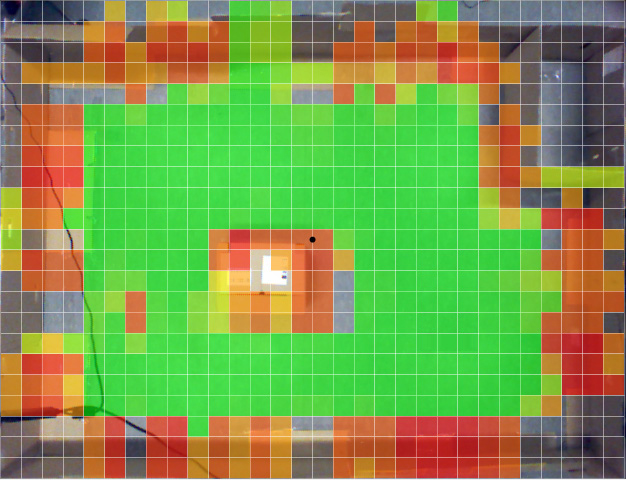
\includegraphics[width=0.6\textwidth]{testresultater/simpel1}}
\end{frame}

\begin{frame}
\frametitle{Yderligere sensor-information}
Informationen fra robottens sensorer kunne give anledning til bedre definition af den verden robotten befinder sig i.
\begin{itemize}
\item Kontinuerlige målinger.
\item Gaussisk fordeling i to dimensioner.
\item Opfattelse af verden i 360$^\circ$.
\begin{itemize}
\item Ydervægge måles kun fra \'en retning.
\item Hjørner kan ikke identificeres
\item Bayes regel har svært ved at stabilisere information når alle målinger højst kan komme fra fire retninger.
\end{itemize}
\end{itemize}
\end{frame}

\begin{frame}
\frametitle{Celle-størrelse}
De afgrænsninger vi har valgt for projektet har medført problemstillinger i forhold til vores målsætning.
\begin{itemize}
\item Alle test udført med 10x10 cm celler.
\item Præcision som målsætning.
\item Reduktion i størrelse er problematisk.
\end{itemize}
\end{frame}

\subsection{Konklusion}

\begin{frame}
\frametitle{Konklusion}
\begin{itemize}
\item Problemformulering:\\
\textit{- Hvordan kan der konstrueres software til en robot, hvis formål er at kortlægge en ukendt verden, forudsat at den til enhver tid kender sin position?}
\pause
\item Robotten kortlægger en ukendt verden og anvender denne information til at navigere i verdenen.
\end{itemize}
\end{frame}